% Unofficial University of Cambridge Poster Template
% https://github.com/andiac/gemini-cam
% a fork of https://github.com/anishathalye/gemini
% also refer to https://github.com/k4rtik/uchicago-poster

\documentclass[final]{beamer}

% ====================
% Packages
% ====================

\usepackage[T1]{fontenc}
\usepackage{lmodern}
\usepackage[size=custom,width=120,height=72,scale=1.0]{beamerposter}
\usetheme{gemini}
\usecolortheme{cam}
\usepackage{graphicx}
\usepackage{booktabs}
\usepackage{tikz}
\usepackage{pgfplots}
\pgfplotsset{compat=1.14}
\usepackage{anyfontsize}
\usepackage{xcolor,mdframed}

% ====================
% Lengths
% ====================

% If you have N columns, choose \sepwidth and \colwidth such that
% (N+1)*\sepwidth + N*\colwidth = \paperwidth
\newlength{\sepwidth}
\newlength{\colwidth}
\setlength{\sepwidth}{0.025\paperwidth}
\setlength{\colwidth}{0.3\paperwidth}
\setlength{\paperwidth}{48in}
\setlength{\paperheight}{36in}
\newcommand{\separatorcolumn}{\begin{column}{\sepwidth}\end{column}}

% ====================
% Title
% ====================

\title{ \Huge{Discover User-App Interactions \& \\  
Solutions to Reducing the Initial User-CPU Latency
}}

\author{\LARGE{Thy Nguyen \and Milon Chakkalakal \and Pranav Thaenraj}}

\institute[shortinst]{\Large{Advisors: Jamel Tayeb, Bijan Arbab, Sruti Sahani, Oumaima Makhlouk, Praveen Polasam, Chansik Im}}

% ====================
% Footer (optional)
% ====================

% \footercontent{ \large{
%   https://github.com/miloncl/System-Usage-Analysis \hfill
%   UCSD HDSI - Intel \hfill
%   {\{tcn002,mlonappa,ethaenra\}@ucsd.edu}}}
% (can be left out to remove footer)

% ====================
% Logo (optional)
% ====================

% use this to include logos on the left and/or right side of the header:
% \logoright{\includegraphics[height=7cm]{logo1.pdf}}
% \logoleft{\includegraphics[height=7cm]{logo2.pdf}}

% ====================
% Body
% ====================

\begin{document}

% Refer to https://github.com/k4rtik/uchicago-poster
% logo: https://www.cam.ac.uk/brand-resources/about-the-logo/logo-downloads
\addtobeamertemplate{headline}{}
{
  \begin{tikzpicture}[remember picture,overlay]
    \node [anchor=north west, inner sep=3cm] at ([xshift=0.0cm,yshift=0.75cm]current page.north west)
    {
\includegraphics[height=5.5cm]{hdsi-intel.jpeg}};
  \end{tikzpicture}

  \begin{tikzpicture}[remember picture,overlay]
    \node [anchor=north west, inner sep=3cm] at ([xshift=110.0cm,yshift=0.75cm]current page.north west)
    {
\includegraphics[height=5.5cm]{ucsd-logo.jpeg}};
  \end{tikzpicture}
}

\begin{frame}[t]
  \begin{columns}[t]
    \separatorcolumn

    \begin{column}{\colwidth}

      \begin{block}{\huge{Abstract}}

        {
          \fontsize{37pt}{44.4pt} \selectfont 
          \begin{itemize}
            \item \textbf{Data loading} icons signal an unpleasant user-wait experience and can tear people away from using an app.
            \item We mitigate the initial latency by collecting system usage data using Intel’s Telemetry and analyzing user-app interaction by EDA, HMM, and LSTM/RNN.
        \end{itemize}
        }
        \begin{figure}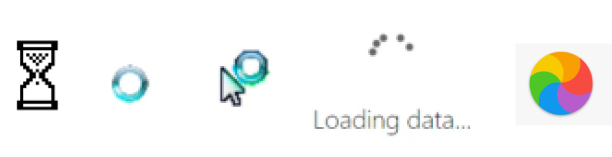
\includegraphics[width=0.6\textwidth, height=5cm]{user-wait.jpeg}\end{figure}

      \end{block}

      \begin{alertblock}{\huge{Methodology of Data Collection}}

        {
          \fontsize{37pt}{44.4pt} \selectfont 
          \begin{itemize}
            \item \textbf{Tools}: Software Development Kit, Environment Server, Intel® System Usage Report framework
            \item \textbf{Purposes} Anonymously gather and analyze data usage from multiple devices. 
          \end{itemize}
        }
        
          \begin{figure}
          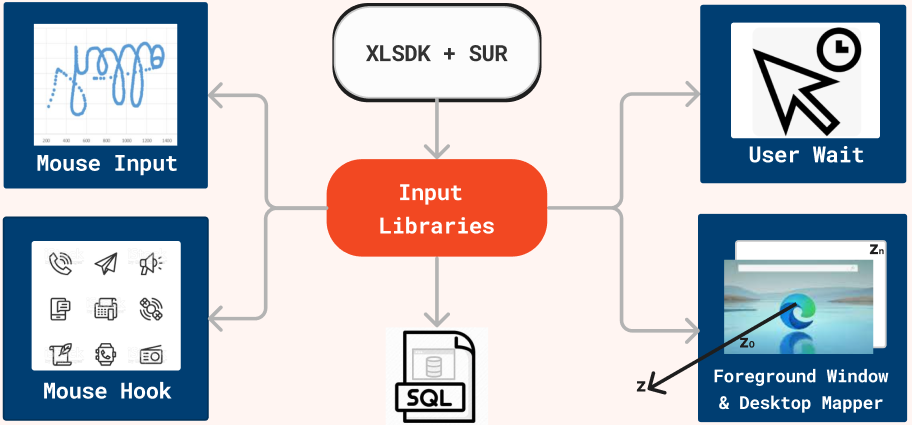
\includegraphics[width=0.96 \textwidth, height=20cm]{data-collection3.jpeg}
          
          % \caption{\large{Mouse Movement, Foreground Window, and Z-axis}}\label{fig:xyz}
          \end{figure}
      \end{alertblock}

      \begin{block}{\huge{Exploratory Data Analysis}}

        {\fontsize{37pt}{44.4pt} \selectfont Chrome is the top frequently used app of this user according to the time measurement in 01/2023}

        \begin{figure}
          \begin{mdframed}[backgroundcolor=gray!5,linecolor=gray!10]
            \centering{\hspace*{-2cm}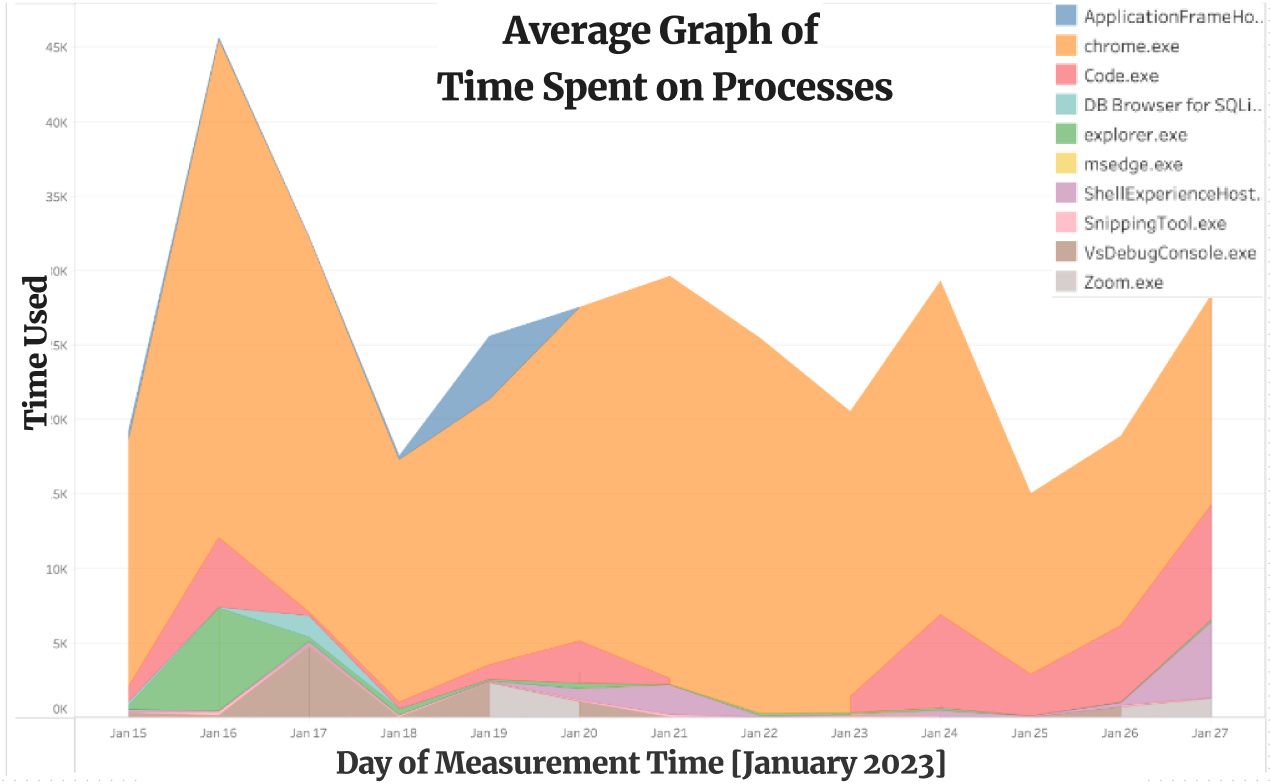
\includegraphics[width=0.85\textwidth, height=18cm]{time-used.jpeg}}
          \end{mdframed}
        \end{figure}

      \end{block}

    \end{column}

    \separatorcolumn

    \begin{column}{\colwidth}

      \begin{exampleblock}{\huge{Methodology of Predictive Tasks}}

        {
          \fontsize{37pt}{44.4pt} \selectfont \heading{Hidden Markov Model  (HMM)}

          \begin{itemize}
            \item \textbf{Problem Statement}: Predict the likelihood of using an app \textit{given} the former sequence of application usage
            \item \textbf{Idea}: Use conditional probability $P(A|B) = \frac{P(A\cap B)}{P(B)}$
            % \item \textbf{HMM Assumptions}:

            \item \textbf{A1. Markov Chain}: Only the \underline{\textit{current}} state $q_{i-1}$ plays the most crucial role in predicting the future in the sequence \\
                  {\centering \textcolor{brown}{$P(q_i = a | q_1q_2...q_{i-1}) = P(q_i= a | q_{i-1})$} \par}

            \item \textbf{A2. Output Independence}: The probability of observing an event $o_i$ only relies on the state $q_i$ that \underline{\textit{directly}} produced $o_i$
\\
                    {\centering \textcolor{brown}{$P(o_i | q_1, ... q_i , ..., q_T, o_1, ..., o_i, ..., o_T) = P(o_i | q_i)$} \par}
                    
                    \begin{figure}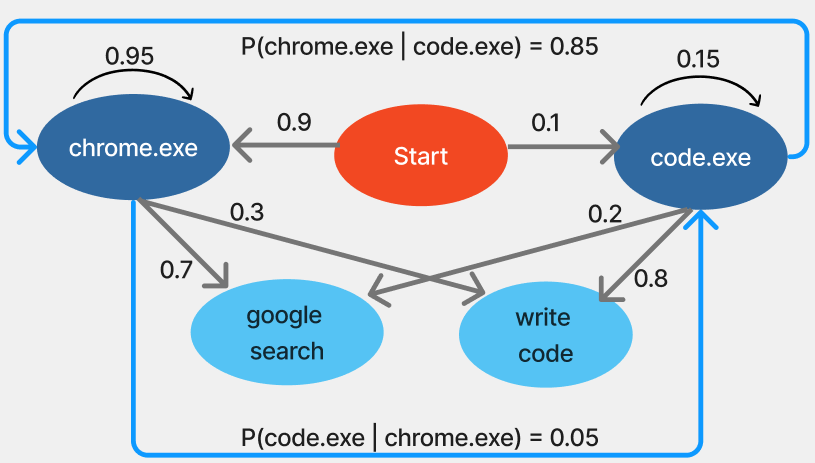
\includegraphics[width=0.75\textwidth, height=16cm]{hmm3.jpeg}\end{figure}
            % \item \textbf{Transition Matrix}: contains the transition probabilities, e.g. the likelihood of moving from one executable to another \\
            %       {\centering \textcolor{brown}{$P($chrome.exe -> cmd.exe$)$ =  $P($cmd.exe | chrome.exe$)$} \par}

            % \item \textbf{Emission Matrix}: contains the emission probabilities, e.g. the likelihood of moving from one executable to another app/tab\\
            %       {\centering \textcolor{brown}{$P($chrome.exe -> Spotify$)$ =  $P($Spotify | chrome.exe$)$} \par}
            
            
            % \item \textbf{Metrics}: Preds==True if within top $n$ probabilities of the app
          \end{itemize}

          \heading{Recurrent Neural Network (LSTM/RNN)}

          \begin{itemize}
            \item \textbf{Problem Statement}: Predict the (total) time usage of an app/tab/recorded process using the past \textit{time-series} data
                  \begin{figure}\hspace*{-2cm}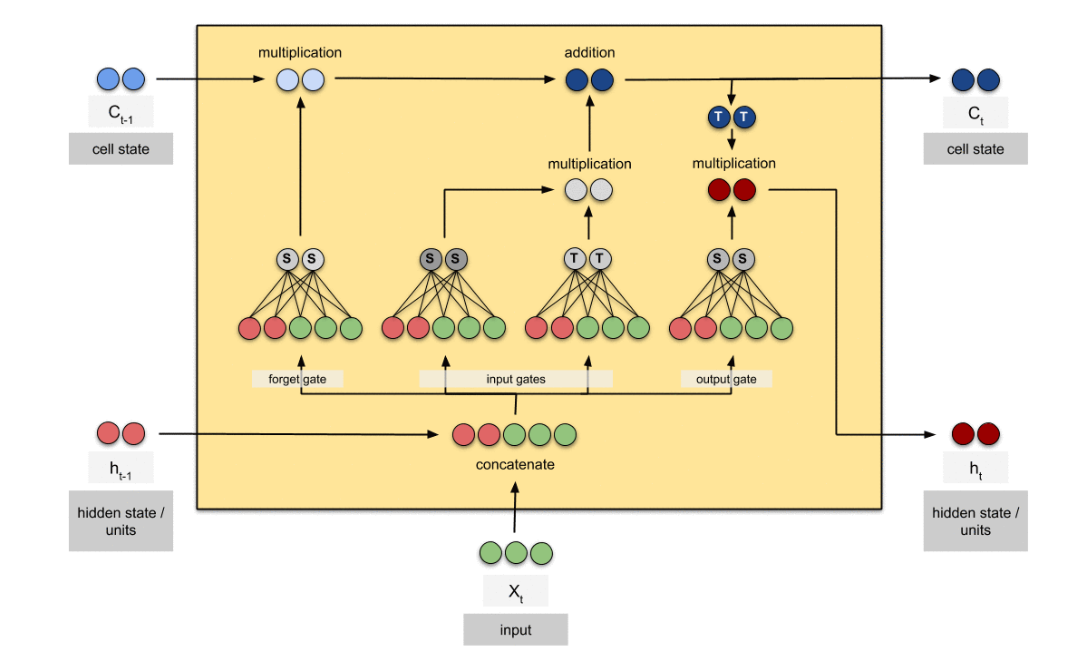
\includegraphics[width=0.8\textwidth, height=22cm]{lstm-lt.jpeg}\end{figure}

            \item \textbf{Feature Engineering}:

                  1. Hourly split daily usage into 24 cols (labeled 0 - 23)\\
                  2. Lookback 3-5 time steps from the current timestamp\\
                  3. One-hot-encoding; Min-Max scaler
            \item \textbf{Experiments}: Train/Test: 80/20, no shuffle; Keras

                  % 1. \textbf{Train/Test}: 80/20, no shuffle\\
                  % 2. \textbf{Metrics}: RMSE, TP/TN/FP/FN, Preds==True if within 1 sec of real vals
            % \item \textbf{Metrics}: RMSE, TP/TN/FP/FN, Preds==True if w/in 1 sec

          \end{itemize} }
      \end{exampleblock}

    \end{column}

    \separatorcolumn

    \begin{column}{\colwidth}

      \begin{block}
        {\huge{Predictive Results}}

        {
          \fontsize{37pt}{44.4pt} \selectfont \centering{\textbf{HMM Metrics}: Preds==True if within top $n$ probabilities
        }}
        % \large{
        %   \begin{table}
        %     \centering
        %     \begin{tabular}{l l l l}
        %       \toprule
        %       \multicolumn{1}{|l|}{\textbf{Num Apps (n)}}                                                                    & \multicolumn{1}{|l|}{\textbf{ACC (User 1)}} & \multicolumn{1}{|l|}{\textbf{ACC (User 2)}} \\
        %       \midrule

        %       \multicolumn{1}{|l|}{\begin{tabular}[c]{@{}l@{}}1 \\  2 \\ 5 \\ 10 \\ 15 \end{tabular}}                    &
        %       \multicolumn{1}{|l|}{\begin{tabular}[c]{@{}l@{}}47.5\%\\ 63.9\%\\ 84.3\% \\ 95.7\% \\ 98.8\%\end{tabular}} &
        %       \multicolumn{1}{|l|}{\begin{tabular}[c]{@{}l@{}}40.1\%\\ 57.5\%\\ 80.0\% \\ 92.6\% \\ 96.6\%\end{tabular}} \\
        %       \midrule
        %     \end{tabular}
        %     \caption[short]{\large {HMM Transition Matrix Performance}}
        %   \end{table}
        % }

        % \large {\textbf{Transition Matrix Results}}\\
        % 1. $n$ = 1,  $\>$  ACC (User 1) = 47.5\%, $\>$ACC (User 2) = 40.1\%\\
        % 2. $n$ = 2,  $\>$  ACC (User 1) = 63.9\%, $\>$ACC (User 2) = 57.5\%\\
        % 3. $n$ = 5,  $\>$  ACC (User 1) = 84.3\%, $\>$ACC (User 2) = 80.0\%\\
        % 4. $n$ = 10, $\>$ACC (User 1) = 95.7\%, $\>$ACC (User 2) = 92.6\%\\
        % 5. $n$ = 15, $\>$ACC (User 1) = 98.8\%, $\>$ACC (User 2) = 96.6\%\\

      %   \begin{figure}
      %     \centering{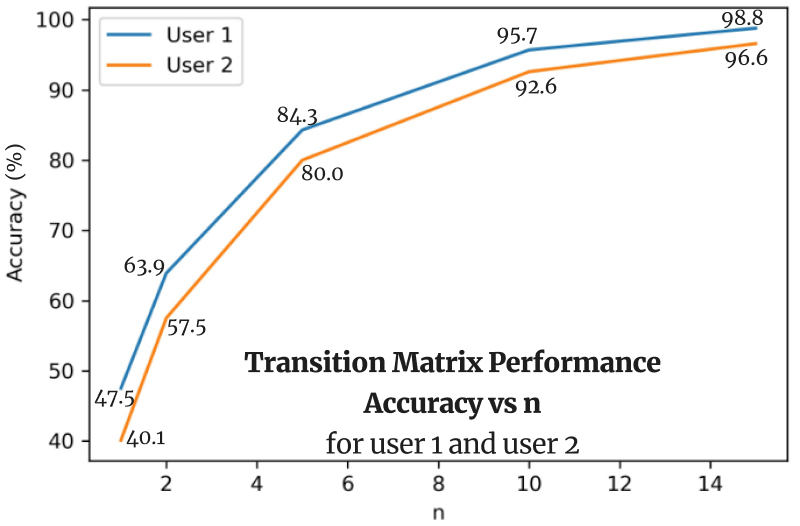
\includegraphics[width=0.6\textwidth, height=15cm]{transition-mt.jpeg}}
      % \end{figure}

      \begin{figure}
        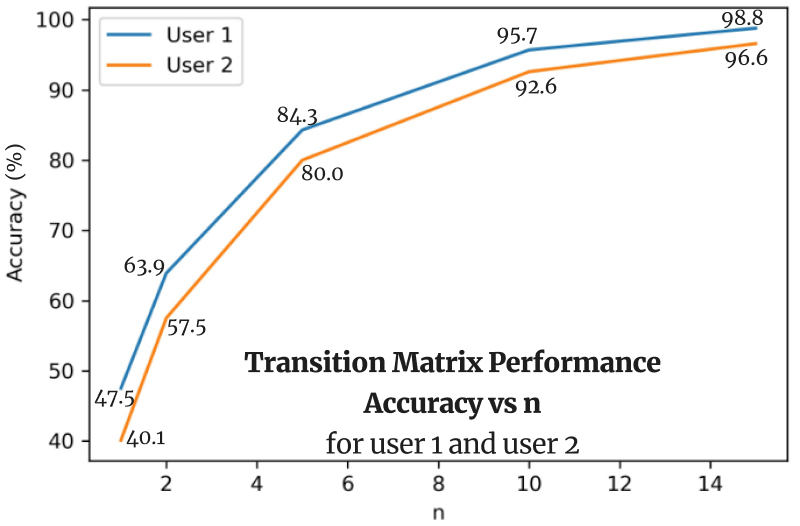
\includegraphics[width=0.475\textwidth, height=15cm]{transition-mt.jpeg}
        \hspace{\fill}
        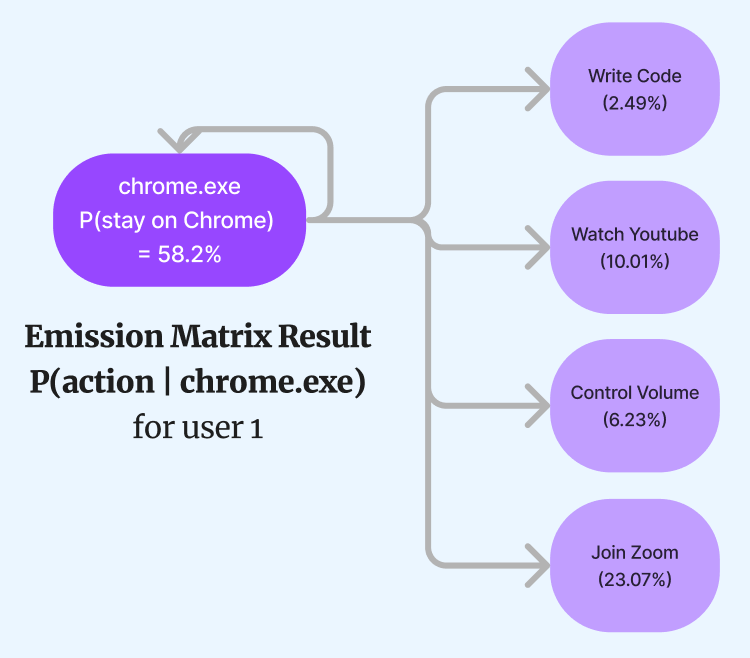
\includegraphics[width=0.48\textwidth, height=15cm]{emission-mt.jpeg}
        \end{figure}


        {
          \fontsize{37pt}{44.4pt} \selectfont \centering{ \textbf{LSTM Metrics}: RMSE, TP/TN/FP/FN, Preds==True if w/in 1 sec
          }}

      %   \begin{figure}
      %     \centering{\hspace*{-2cm}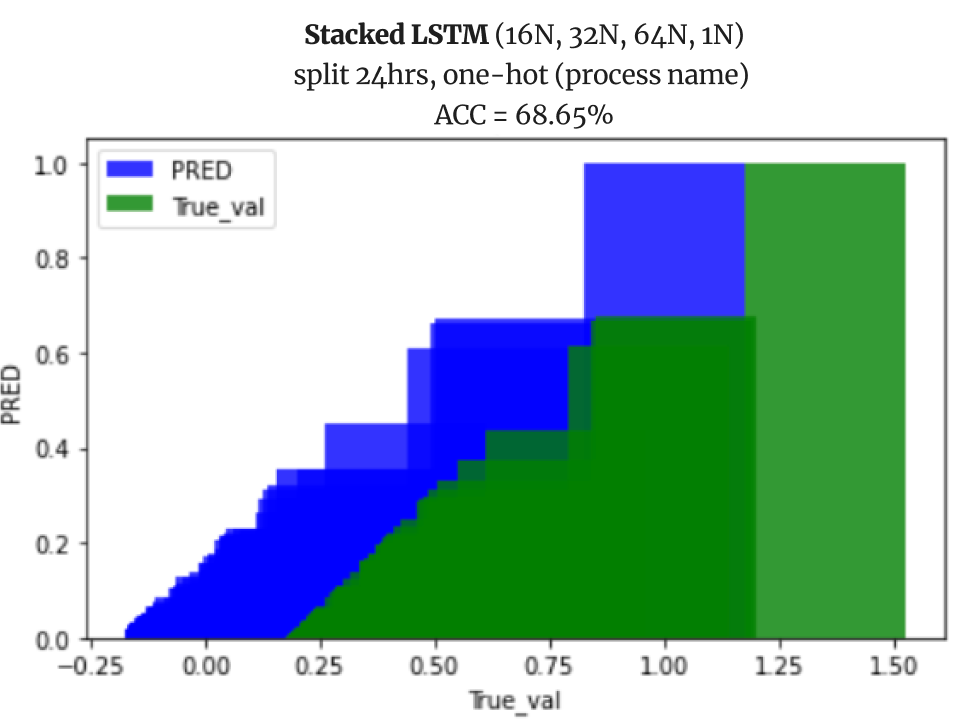
\includegraphics[width=0.8\textwidth, height=20cm]{stacked-lstm.jpeg}}
      % \end{figure}

      \begin{figure}
        \centering{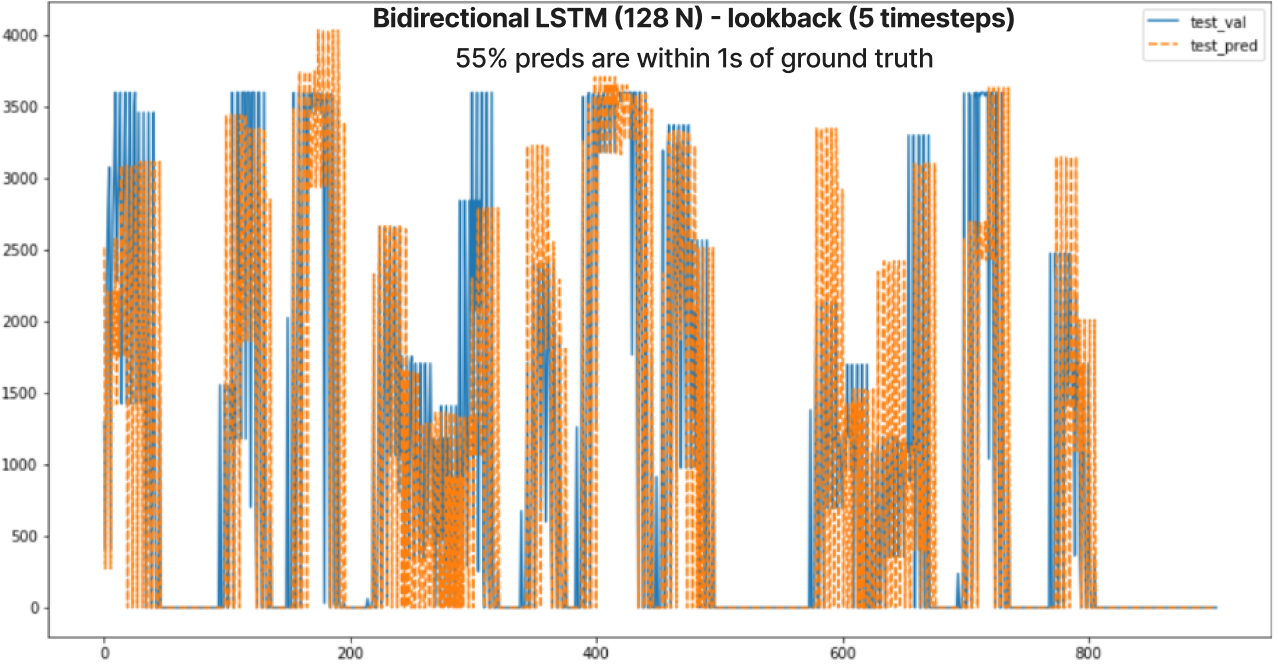
\includegraphics[width=0.98\textwidth, height=18cm]{bi-lstm.jpeg}}
      \end{figure}
      \large{\textbf{LSTM/RNN Performance}}\vspace*{-\baselineskip}
        \large{
          \begin{table}
            \centering
            \begin{tabular}{l l l l}
              \toprule
              \multicolumn{1}{|l|}{\textbf{Model}}                                                                                                         & \multicolumn{1}{|l|}{\textbf{Design (N=nodes)}} & \multicolumn{1}{|l|}{\textbf{Eval Bins/Criteria}} & \multicolumn{1}{|l|}{\textbf{Performance}} \\
              \midrule

              \multicolumn{1}{|l|}{\begin{tabular}[c]{@{}l@{}}Vanilla LSTM \\  > Split Hourly \\ > OH(Process Name)\end{tabular}}                          &
              \multicolumn{1}{|l|}{\begin{tabular}[c]{@{}l@{}}Input RNN (64N)\\ Hidden Dense (4N)\\ Output Dense (1N)\end{tabular}}                        &
              \multicolumn{1}{|l|}{\begin{tabular}[c]{@{}l@{}}[0, 0.01] \\ (0.01, 0.02]  \\ (0.02, 0.2] \\ (0.2, max] \end{tabular}}                            &
              \multicolumn{1}{|l|}{\begin{tabular}[c]{@{}l@{}}TP = 691, TN = 0\\ FP = 65, FN = 0 \\ ACC = $\approx$ 91.4\% \end{tabular}}                                                                                                                                                            \\
              \midrule

              \multicolumn{1}{|l|}{\begin{tabular}[c]{@{}l@{}}Stacked LSTM \\  > Split Hourly \\ > OH(Process Name)\end{tabular}}                          &
              \multicolumn{1}{|l|}{\begin{tabular}[c]{@{}l@{}}Input LSTM (16N)\\ Hidden LSTM (32N)\\ Hidden Dense (64N) \\ Output Dense (1N)\end{tabular}} &
              \multicolumn{1}{|l|}{\begin{tabular}[c]{@{}l@{}}[0, 0.01] \\ (0.01, 0.02]  \\ (0.02, 0.2] \\ (0.2, max] \end{tabular}}                            &
              \multicolumn{1}{|l|}{\begin{tabular}[c]{@{}l@{}}TP = 467, TN = 52\\ FP = 13, FN = 224 \\ ACC = $\approx$ 68.65\% \end{tabular}}                                                                                                                                                        \\
              \midrule

              

              \multicolumn{1}{|l|}{\begin{tabular}[c]{@{}l@{}}Stacked LSTM \\  > Split Hourly \\ > Lookback(5 timesteps)\end{tabular}}                     &
              \multicolumn{1}{|l|}{\begin{tabular}[c]{@{}l@{}}Input LSTM (50N)\\ Hidden LSTM (50N)\\ Output Dense (1N)\end{tabular}}                       &
              \multicolumn{1}{|l|}{\begin{tabular}[c]{@{}l@{}}Preds==True \\ if abs(diff) <= 3mins \end{tabular}}                                          &
              \multicolumn{1}{|l|}{\begin{tabular}[c]{@{}l@{}} RMSE = 1134.68 \\ ACC = $\approx$ 27\% \end{tabular}}                                                                                                                                                                                 \\
              \midrule
            \end{tabular}
            \caption[short]{\large {LSTM/RNN Performance}}
          \end{table}
        } 
        
      \end{block}

      \begin{block} {\huge{Conclusions}}     
        {
          \fontsize{37pt}{44.4pt} \selectfont
                \begin{itemize} 
                  \item We should collect data \underline{\textit{continuously}} and \underline{\textit{consistently}} to achieve high accuracies in detecting patterns of user behaviors
                  \item The results help infer daily app sequence and time usage, so we can develop a script to process background tasks and utilize \textit{Task Manager} to open the next app 2-3 mins beforehand 
                \end{itemize}
        }
      \end{block}

    \end{column}

    \separatorcolumn
  \end{columns}
\end{frame}

\end{document}